The information recieved from the detector is in the format of detector hits and electrical signals, which is not directly suitable for physics analyses. In this chapter we introduce the reconstruction and identification of physics particles involved in this analysis, based on the detector-level information. 

\vspace{0.3cm}
The Particle-Flow algorithm~\cite{ob_pf} is used for event and particle reconstructions.

\section{Particle Flow Algorithm}
The PF algorithm starts from reconstructing the basic PF elements including the trajectories of charged particles, electron/muon tracks and calorimeter clusters, based on the information collected from each subsystem of the detector. Then a linking algorithm is used to form a block of these PF elements possibly related to a single physics object. Afterwards, the particle constructions and identifications are processed based on the blocks. The constructions of the PF elements are described briefly as below.

\subsection{Charged-particle tracks and vertices}
The construction of charged-particle tracks provides supports for particle reconstructions and identifications, including the measurement of the momentum of energetic and isolated muons, identification of energetic and isolated hadronic $\tau$ decays, and tagging b quark jets. A combinatorial track finder based on Kalman Filtering (KF) is used for track construction~\cite{ob_trackconst1,ob_trackconst2}. It starts with a few hits compatible with a charged-particle trajectory in the tracking system; and then finds hits from all the tracker layers along this charged-particle trajectory; and finally performs fitting to determine the trajectory and the particle properties including origin, transverse momentum and direction. To increase the reconstruction efficiency and suppress the fake rate, the combinatorial track finder was applied in several successive iterations.

\vspace{0.3cm}
The vertex reconstruction aims at determine the locations of all the proton-proton interactions and uncertainties in each event. The vertex reconstruction uses the information of the reconstructed charged-particle tracks. After determining the candidate vertices with the deterministic annealing (DA) algorithm and fitting them with at least two matched tracks using an adaptive vertex fitter, good vertices are selected with quality criteria including being consistent with the collision region (referred to as beam spots) and matched to a minimum of four tracks. The primary vertex of an event is considered to be the vertex with the largest sum of the squared track momenta. And the other vertices are regarded as pileup vertices. Figure~\ref{fig:ob_Nvertex} shows the vertices number distribution for the data collected in 2016.
\begin{figure}[htbp]
\begin{center}
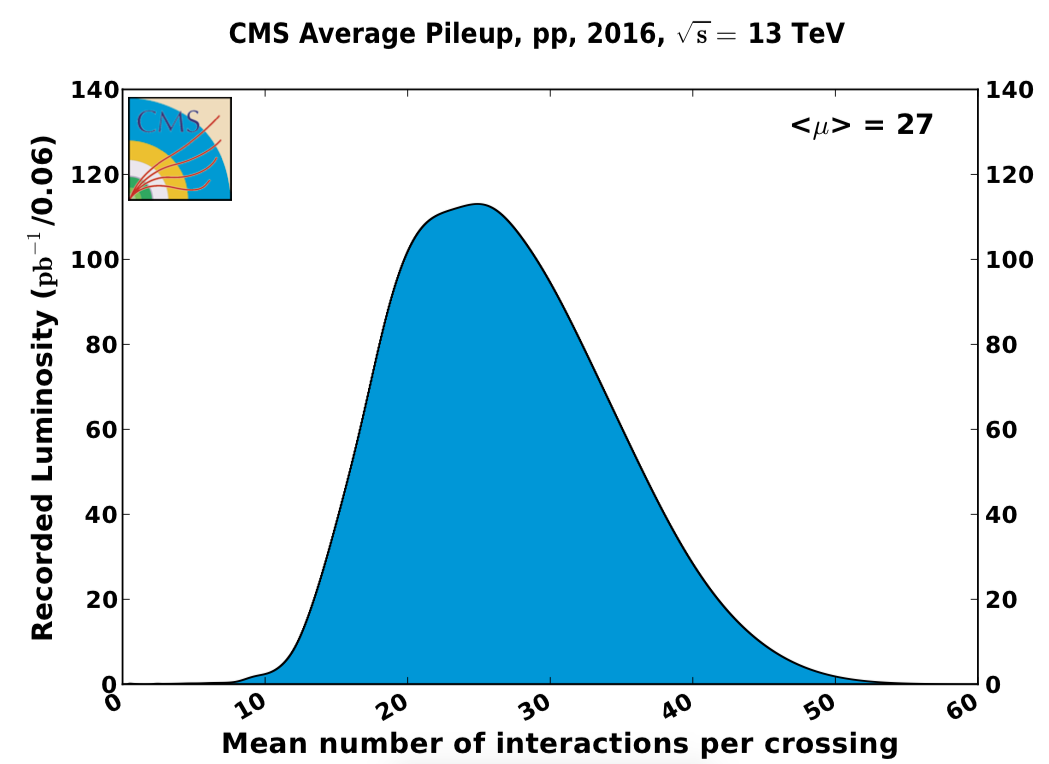
\includegraphics[width=0.72\linewidth]{figures/ob_Nvertex.png}
\caption{Number of interactions per bunch crossing for data collected in 2016.}
\label{fig:ob_Nvertex}
\end{center}
\end{figure}

\subsection{Calorimeter clusters}
The calorimeter clustering serves four purpose in general: detect and measure the energy and direction of stable neutral particles; separate these neutral particles from charged hadron energy deposits; reconstruct and identify electrons and all accompanying bremsstrahlung photons; and help the energy measurement of charged hadrons for which the track parameters were not determined accurately. An algorithm is developed and the clustering process is performed seperately for EB, EE, ES, HB and HE. Firstly cluster seeds are selected as calorimeter cells with deposited energy larger than a threshold and its neighbouring cells. The topological clusters then spread from the seed to the nearby cells with energy beyond cerntain thresholds. Finally a fitting for each topological cluster is performed based on an expectation-maximization algorithm to evaluate position and amplitude of the particle clusters.

\subsection{Tracks for electrons}
Because of the significant tracker thickness, most of the electrons emit considerable fraction of their energy in the form of bremsstrahlung photons before reaching the ECAL. To reconstruct the properties of an electron, the energy of the bremsstrahlung photons in ECAL must be taken into account as well, apart from the energy deposited by the final electron. A tracker-based electron seeding method was developed

\subsection{Tracks for muons}


\section{Electron}

\subsection{Electron Reconstruction}
\subsection{Electron Identification}
\section{Photon}
\subsection{Photon Reconstruction}
\subsection{Phoon Identification}
\section{Muon}
\subsection{Muon Reconstruction}
\subsection{Muon Identification}
\subsubsection{Muon ID}
\subsubsection{Muon Isolation}
\section{Missing Transverse Energe (MET)}
